\documentclass[english]{article}

\usepackage[utf8]{inputenc}
\usepackage{graphicx}
\graphicspath{ {images/} }
\usepackage[margin=2.5cm]{geometry}
\usepackage{eso-pic}
\usepackage{hyperref}
\usepackage{wrapfig}
\usepackage{lipsum}
\usepackage{array}
\usepackage{enumitem}
\usepackage{qtree}
\usepackage{color}
\usepackage{forest}
\usepackage{tikz}
\usepackage{grffile}
\usepackage{babel}
\usepackage{listings}
\usepackage{hyperref}
\hypersetup{
    colorlinks=true,
    linkcolor=blue,
    filecolor=magenta,      
    urlcolor=cyan,
}
 
\urlstyle{same}

\begin{document}
\begin{titlepage}
	\begin{center}
		\begin{figure}[t]
			\centering
			
\includegraphics[width=350px]{logo.PNG}
		\end{figure}
		\begin{center}
			\textsc{\LARGE COS 301}
		\end{center}
		\begin{center}		
			\textsc{\LARGE V3D Graph Visualizer: User Manual}		
		\end{center}
		
		\begin{flushright} \large
			App-Synth \newline \emph{} \newline
		\end{flushright}


	\end{center}
\end{titlepage}

\newpage
\pagenumbering{arabic}
\thispagestyle{empty}
\tableofcontents
\clearpage

\setcounter{page}{1}

\section{Introduction}
\subsection{System Overview}
The V3D Digraph Visualizer is a graph visualization tool that allows users to perceive the information contained within digraphs which will be defined using the set of triples notations specified by Barla-Szabo in a 3D environment. The system will allow users to visualize and interact with the graph models in a 3D space. The system will consist of a mobile and a desktop application. The mobile application will allow the user to visualise the graph in a 3D space with the use of a mobile virtual reality headset, while the desktop application displays the visualisation for observers.

\subsection{System Configuration}
\begin{flushleft}
In order to make use of the system, ensure that you have all of the necessary hardware and software. These include:

\begin{itemize}
  \item A desktop or laptop computer
  \item A mobile device running Android Jelly Bean (version 4.1.1) or newer
  \item A mobile VR (Virtual Reality) headset (Google Cardboard is recommended)
  \item The TeamViewer Quick Support mobile application
  \item The TeamViewer desktop application
  \item An internet connection to which both the mobile device and desktop are connected
  \item Google Cardboard Mobile App
\end{itemize}
\end{flushleft}
\section{Installation}
The installation file for the mobile application can be obtained from the following link: (url to git apk). Once the installation file has been downloaded successfully, navigate to the Downloads folder on your mobile device, locate the installation file named V3D.apk and proceed to install the application. If the installation was downloaded on another device, simply copy the file over to the device you intend to use, navigate to the installation file and proceed to install the application. The TeamViewer QuickSupport mobile application can be downloaded directly from the Google Play Store and the TeamViewer desktop application can be downloaded from the TeamViewer Website using the link provided above 
 
\section{Getting Started}
Once all of the necessary hardware and software has been obtained, start the TeamViewer application on the mobile device. You will be presented with a screen which contains your TeamViewer ID. This ID will be used to connect to your TeamViewer Desktop application. Open the TeamViewer Desktop application. Under the “Control Remote Computer” section you should see an input field titled “Partner ID”. Enter the TeamViewer ID obtained from your mobile device and click the button labelled “Connect to Mobile Partner”. A message should appear on your mobile device requesting a connection to your desktop. Select the “Allow” option. The TeamViewer application should minimize on your mobile device and you should now see an emulation of your mobile device screen on your desktop computer. If TeamViewer does not connect, ensure that your mobile device and desktop computer are connected to the same network. Once this has been done, you may start the V3D application. Once the application has launched, a message should appear requesting access to the mobile devices’ internal storage. Select the “Allow” option. You may now place the mobile device inside the VR headset.

\section{Usage} 
\subsection{Interactions}
A lot of the interactions within the virtual reality environment will be performed using the reticle which is positions at the center of the screen. To interact with a button or a control on the screen, simply position the reticle over it. The reticle will expand into a circle when interacting with a button or control and retract back into a dot when moved away from a button / control.

\subsection{Start Menu}
Once the application is running, you will be presented with a menu consisting of 3 options within the virtual reality environment. The first option is titled “Get Started” and should be located directly in front of you. Select this option if you wish to create your own directed graph within the virtual environment. The second option is titled “Create Graph” and should be located to your left. Select this option if you wish to create a new graph specification using the online V3D graph creator. The third option is titled “Load Existing Graph” and should be located to your right. Select this option if you already have a graph specification file on your mobile device which you wish to visualise. To select an option, position the reticle over the rectangular object underneath the appropriate heading. The box should begin to change colour and the reticle should form a circular shape. Maintain this position until the VR environment changes. More detail about each option will be provided below.

\subsection{Get Started}
Once you have selected this option, you should be presented with the screen below. The buttons towards the bottom of the screen are graph controls used to alter the position of the graph by rotating the graph in different directions using the upward, downward, left and right facing arrow buttons and zooming in and out using the “+” and “-” buttons. The button located towards the top-left corner of the screen is used to go back to the main menu. The button located towards the top-right hand side of the screen with a lightning bolt shape is used to add a new node to the scene. The checkbox which is also located towards the top-right corner of the screen is used to switch between edit mode and view mode. When the checkbox is checked, edit mode will be activated. In this mode, the user can add nodes to the graph and create edges between existing nodes. Then the checkbox is not checked, view mode will be activated. In this mode, the user may only view the graph and may not create any nodes or any relationships. 

\subsubsection{Create Graph}
\paragraph{Create Node: }
In order to create a graph node, hover over the “Create Node” button which has a lightning bolt icon on it for 2 seconds using the reticle. A red graph node should appear close to the centre of the screen. You can pick up a graph node by hovering over it for 2 seconds using the reticle. The node should turn blue and become attached to the reticle and you may now move the node around in the scene. To drop a node, simply hold your head still for 2 seconds. The node should return to its original colour and become detached from the reticle. To create a relationship between two nodes, pick up the node you wish to be the parent node and move it towards the node you wish to connect it to until the two nodes touch. This will create an edge between the two nodes with an arrow pointing from the parent node to the child node.

\paragraph{Remove Node: }
In order to remove a node, pick up the node using the reticle and position the node over the green button with an "X" on it. Hold the node in this position for 2 seconds and it should be removed from the graph. With the removal of the node, any edges which were connected to the node will also be removed.

\paragraph{Save Graph: }
Once you have finished creating the graph, you can save it to a file which can be used to load the graph at a later stage. To save a graph, hover over the button towards the top right corner of the screen. Maintain this position for 2 seconds and the application should navigate back to the start menu. At this point, your graph file should be saved to the Downloads directory on your mobile device.

\subsection{Load existing graph}
This option allows you to load a graph file that has already been stored on the mobile device. Upon selecting this option, you will see a grid of rectangles each with the name of any graph specifications which were found on your device. Use the reticle to select the desired graph, and you should be taken to a scene which contains a visualisation of the graph. The controls, buttons and functionality in this scene are identical to those mentioned in the section above titled “Get Started”. You will have the ability to view the graph, rotate it, zoom in and out and also create and remove nodes and relationships and save the graph to a graph specification file.

\subsection{Create/Edit and Download Graph Files Online Interface}


\includegraphics[width=450px]{InterfaceScreenshots/InterfaceCoverPage.PNG}

\subsubsection{Overall Interface Description}
The user is able to create their own graphs and edit existing graph files without having to be familiar with the format the application uses. The user can interact with a web interface to do so.

\subsubsection{Creating a New Graph}

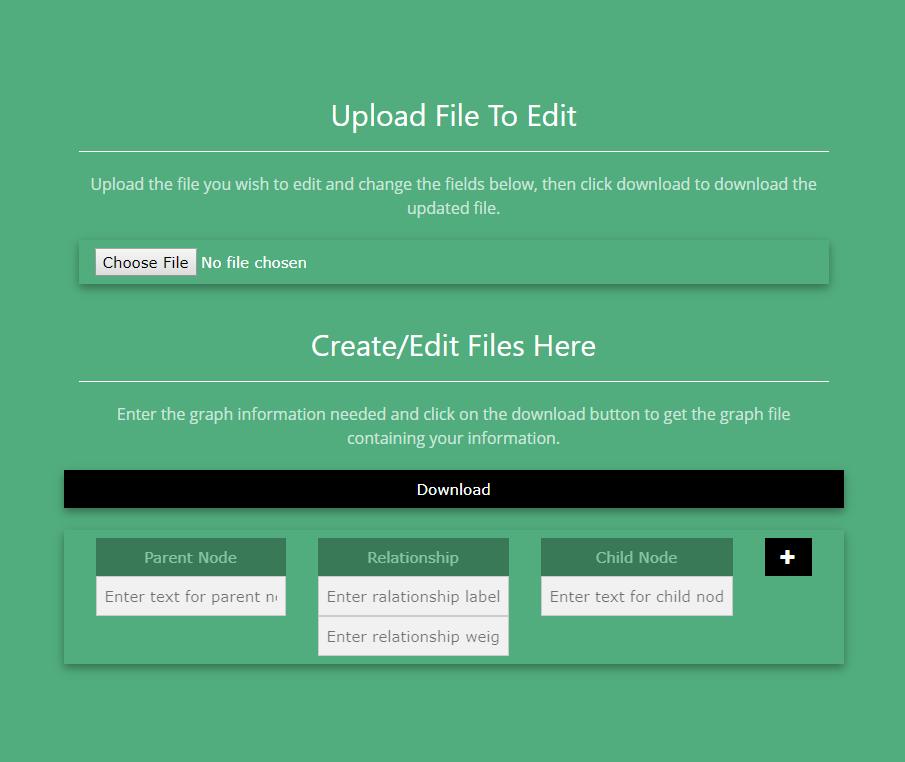
\includegraphics[width=500px]{InterfaceScreenshots/EmptyInfo.PNG}

\subsubsection{Enter Node Name and Relationship Information}
To create a new graph the first step is to insert the node information required. This is done by inserting a parent node name, the relationship information it has with another node and finally the node with which this relationship is shared. The direction of the relationship goes from parent to child. Once this is entered, click the add button to add the nodes and the relationship.

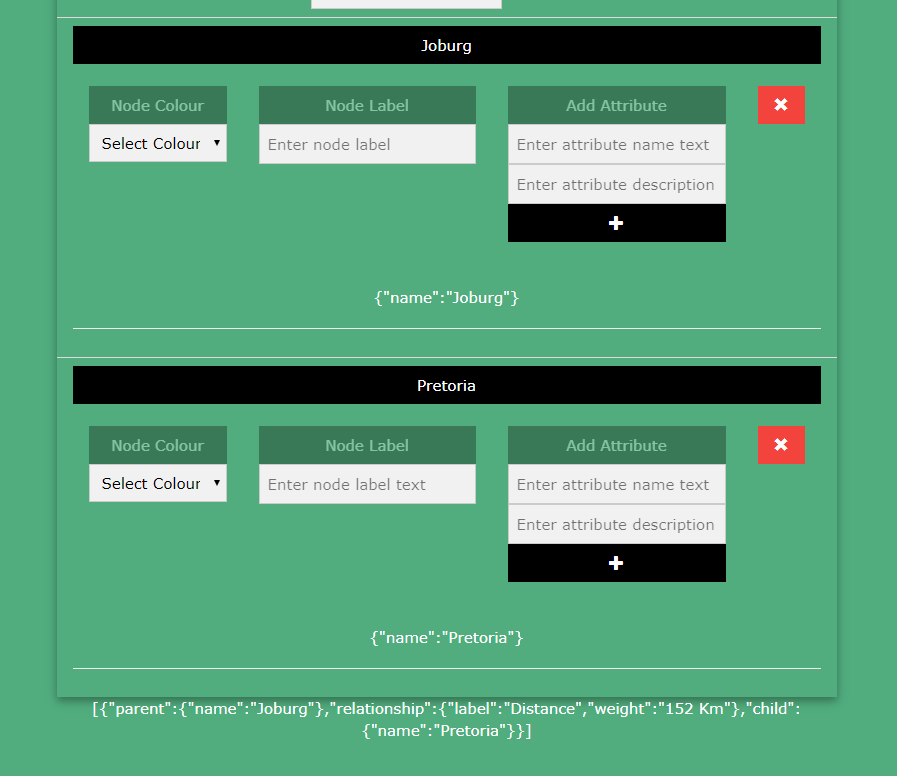
\includegraphics[width=500px]{InterfaceScreenshots/NewNodes.PNG}

\subsubsection{Inserting Node Information}
After adding the node names and relationship information. The nodes will appear bellow with input areas that allow the user to enter node specific information. These include the colour the user wishes the node to appear in, its label and an area to add attributes to the node that the user deems appropriate. Nodes can be removed at any time the user decides by clicking the remove button in red.

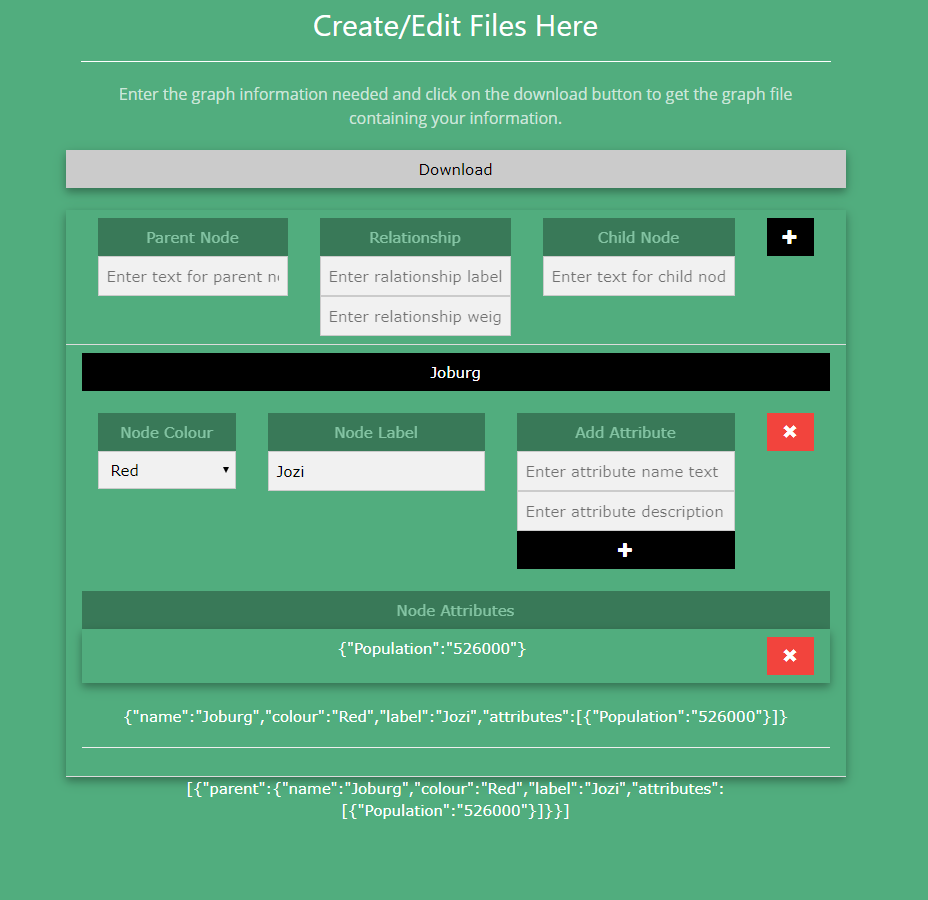
\includegraphics[width=500px]{InterfaceScreenshots/AttributeAdded.PNG}

\subsubsection{Adding and Removing Node Attributes}
There are Two available inputs for the user to enter node attributes. One for the attribute name and the other for the attribute value. Once the user inserts the required information, the node attributes will appear beneath with the heading of 'Node Attributes'. The user can remove node attributes by clicking the red remove button that is placed to the right of it.

\subsubsection{Editing an Existing Graph File}
In order to select an existing graph, the user must click on the 'Choose File' button. Once clicked the user will be able to select a file to edit. After selecting a file the interface will load all the graph information into the page. The user can now change or add information and click the download button to get the updated file.

\subsubsection{Downloading The File With Information Entered}
To download the file the user has edited or created, the user must click on the download button. This is placed towards the top of the input areas on the web interface.

\end{document}
